\documentclass[11pt
  , a4paper
  , article
  , oneside
  %  , twoside
  , showtrims
 % , draft
]{memoir}



\usepackage{essdocs}
\usepackage[numbers]{natbib}
\usepackage[autostyle]{csquotes}

\setsecnumdepth{subsection}


\begin{document}
%\frontmatter
%% ESS Document Description
%%
\essdocdesc{Engineering Manual}

%% ESS Document Number
%%
\essdocnum{ESS-XXXXXXXX}

%% Date
%%
\date{\today}

%% ESS Document Revision Number
%%
\essdocrev{0.2}

%% ESS Document State
%%
\essdocstate{Early Draft}

%% ESS Document Classification
%%
\essdocclass{ESS Use Only}

%% Document Title
%%
\title{ICS Engineering Manual}
\subtitle{for MRF cPCI-EVG-230}
%% Document Author(s), if more than one author,
%% use \newline instead of \\ or \linebreak in order to seperate them
\author{Javier Cereijo Garcia \newline Jeong Han Lee }

%% Document Reviewer(s) if more than one reviewer,
%% use \newline instead of \\ or \linebreak in order to seperate them
%\reviewer{Timo Korhonen (Chief Engineer) \newline Timo Korhonen (Chief Engineer)}
\reviewer{TBD}
%% Document Owner(s) if more than one owner,
%% use \newline instead of \\ or \linebreak in order to seperate them
\owner{ICS}

%% Document Approver(s) if more than one approver,
%% use \newline instead of \\ or \linebreak in order to seperate them
\approver{ICS}

\showtrimson

\esstitle
\newpage
\tableofcontents
\newpage

%\mainmatter


%%% Actual Document Start at below
\chapter{Overview}
At European Spallation Source (ESS), Integrated Control System (ICS) uses the Micro Research Finland (MRF) Timing System{\footnote{\url{http://www.mrf.fi/}}} as its timing system of the ESS site. The consistent and up-to-date engineering manual is essential for the ESS Timing system.

\section{Scope}
\begin{itemize}
\item This document identifies one of the MRF Timing Event Generators (EVG) that needs to be configured for an ESS subsystem that needs synchronous frequencies, trigger signals and sequences of events \cite{MRFEVENTGENERATOR}.
\item This document provides the generic description of the MRF cPCI-EVG-230. In addition, it affords the minimal, essential, and generic information for the system configuration.
\item The purpose of this document is to describe the engineering procedure and troubleshooting about how the MRF cPCI-EVG-230 board will be integrated in cooperation with the new ESS EPICS environment (E3).
\item This document attempts to maintain consistency with existing ESS Timing system hardware as far as possible.
\end{itemize}
\textbf{Note that this is a very early draft document and should be updated as development progresses.}

\section{Target Audience}
This document is targeted to ICS engineers and technical stakeholders of the ESS timing system. It is assumed that the target audience has a technical background in the MRF Timing System, the EPICS development, and a Linux environment.

\chapter{System Description}
MRF Event Generator Modular Register Map Firmware document \citep[see][p4]{MRFEVENTGENERATOR} explained Event Generators and wrote :
\blockquote{\textit{The Event Generator is responsible of creating and sending out timing events to an array of Event Receivers.
High configurability makes it feasible to build a whole timing system with a single Event Generator without external counters etc.
Events are sent out by the event generator as event frames (words) which consist of an eight bit event code and an eight bit distributed bus data byte. The event transfer rate is derived from an external RF clock or optionally an on-board clock generator. The optical event stream transmitted by the Event Generator is phase locked to the clock reference.
There are several sources of events: trigger events, sequence events, software events and events received from an upstream Event Generator. Events from different sources have different priority which is resolved in a priority encoder.
In addition to events the Event Generator enables the distribution of eight simultaneous signals sampled with the event clock rate, the distributed bus. Distributed bus signals may be provided externally or generated on-board by programmable multiplexed counters.}}

In the phase of operation ESS will use a MTCA-EVM-300 as a master event generator, but at the moment several EVG architectures are being used for different purposes:
\begin{itemize}
\item VME-EVG-230
\item MTCA-EVM-300
\item cPCI-EVG-230
\end{itemize}
% I don't know if this list is complete.

The scope of this document is to cover the cPCI-EVG-230 board.


\section{cPCI-EVG-230}
Figure~\ref{fig:cpci-evg230} shows the cPCI-EVG-230 card with rough physical dimensions $100\times 160~\mathrm{mm}{}^2$.

\begin{figure}[!htb]
  \centering
  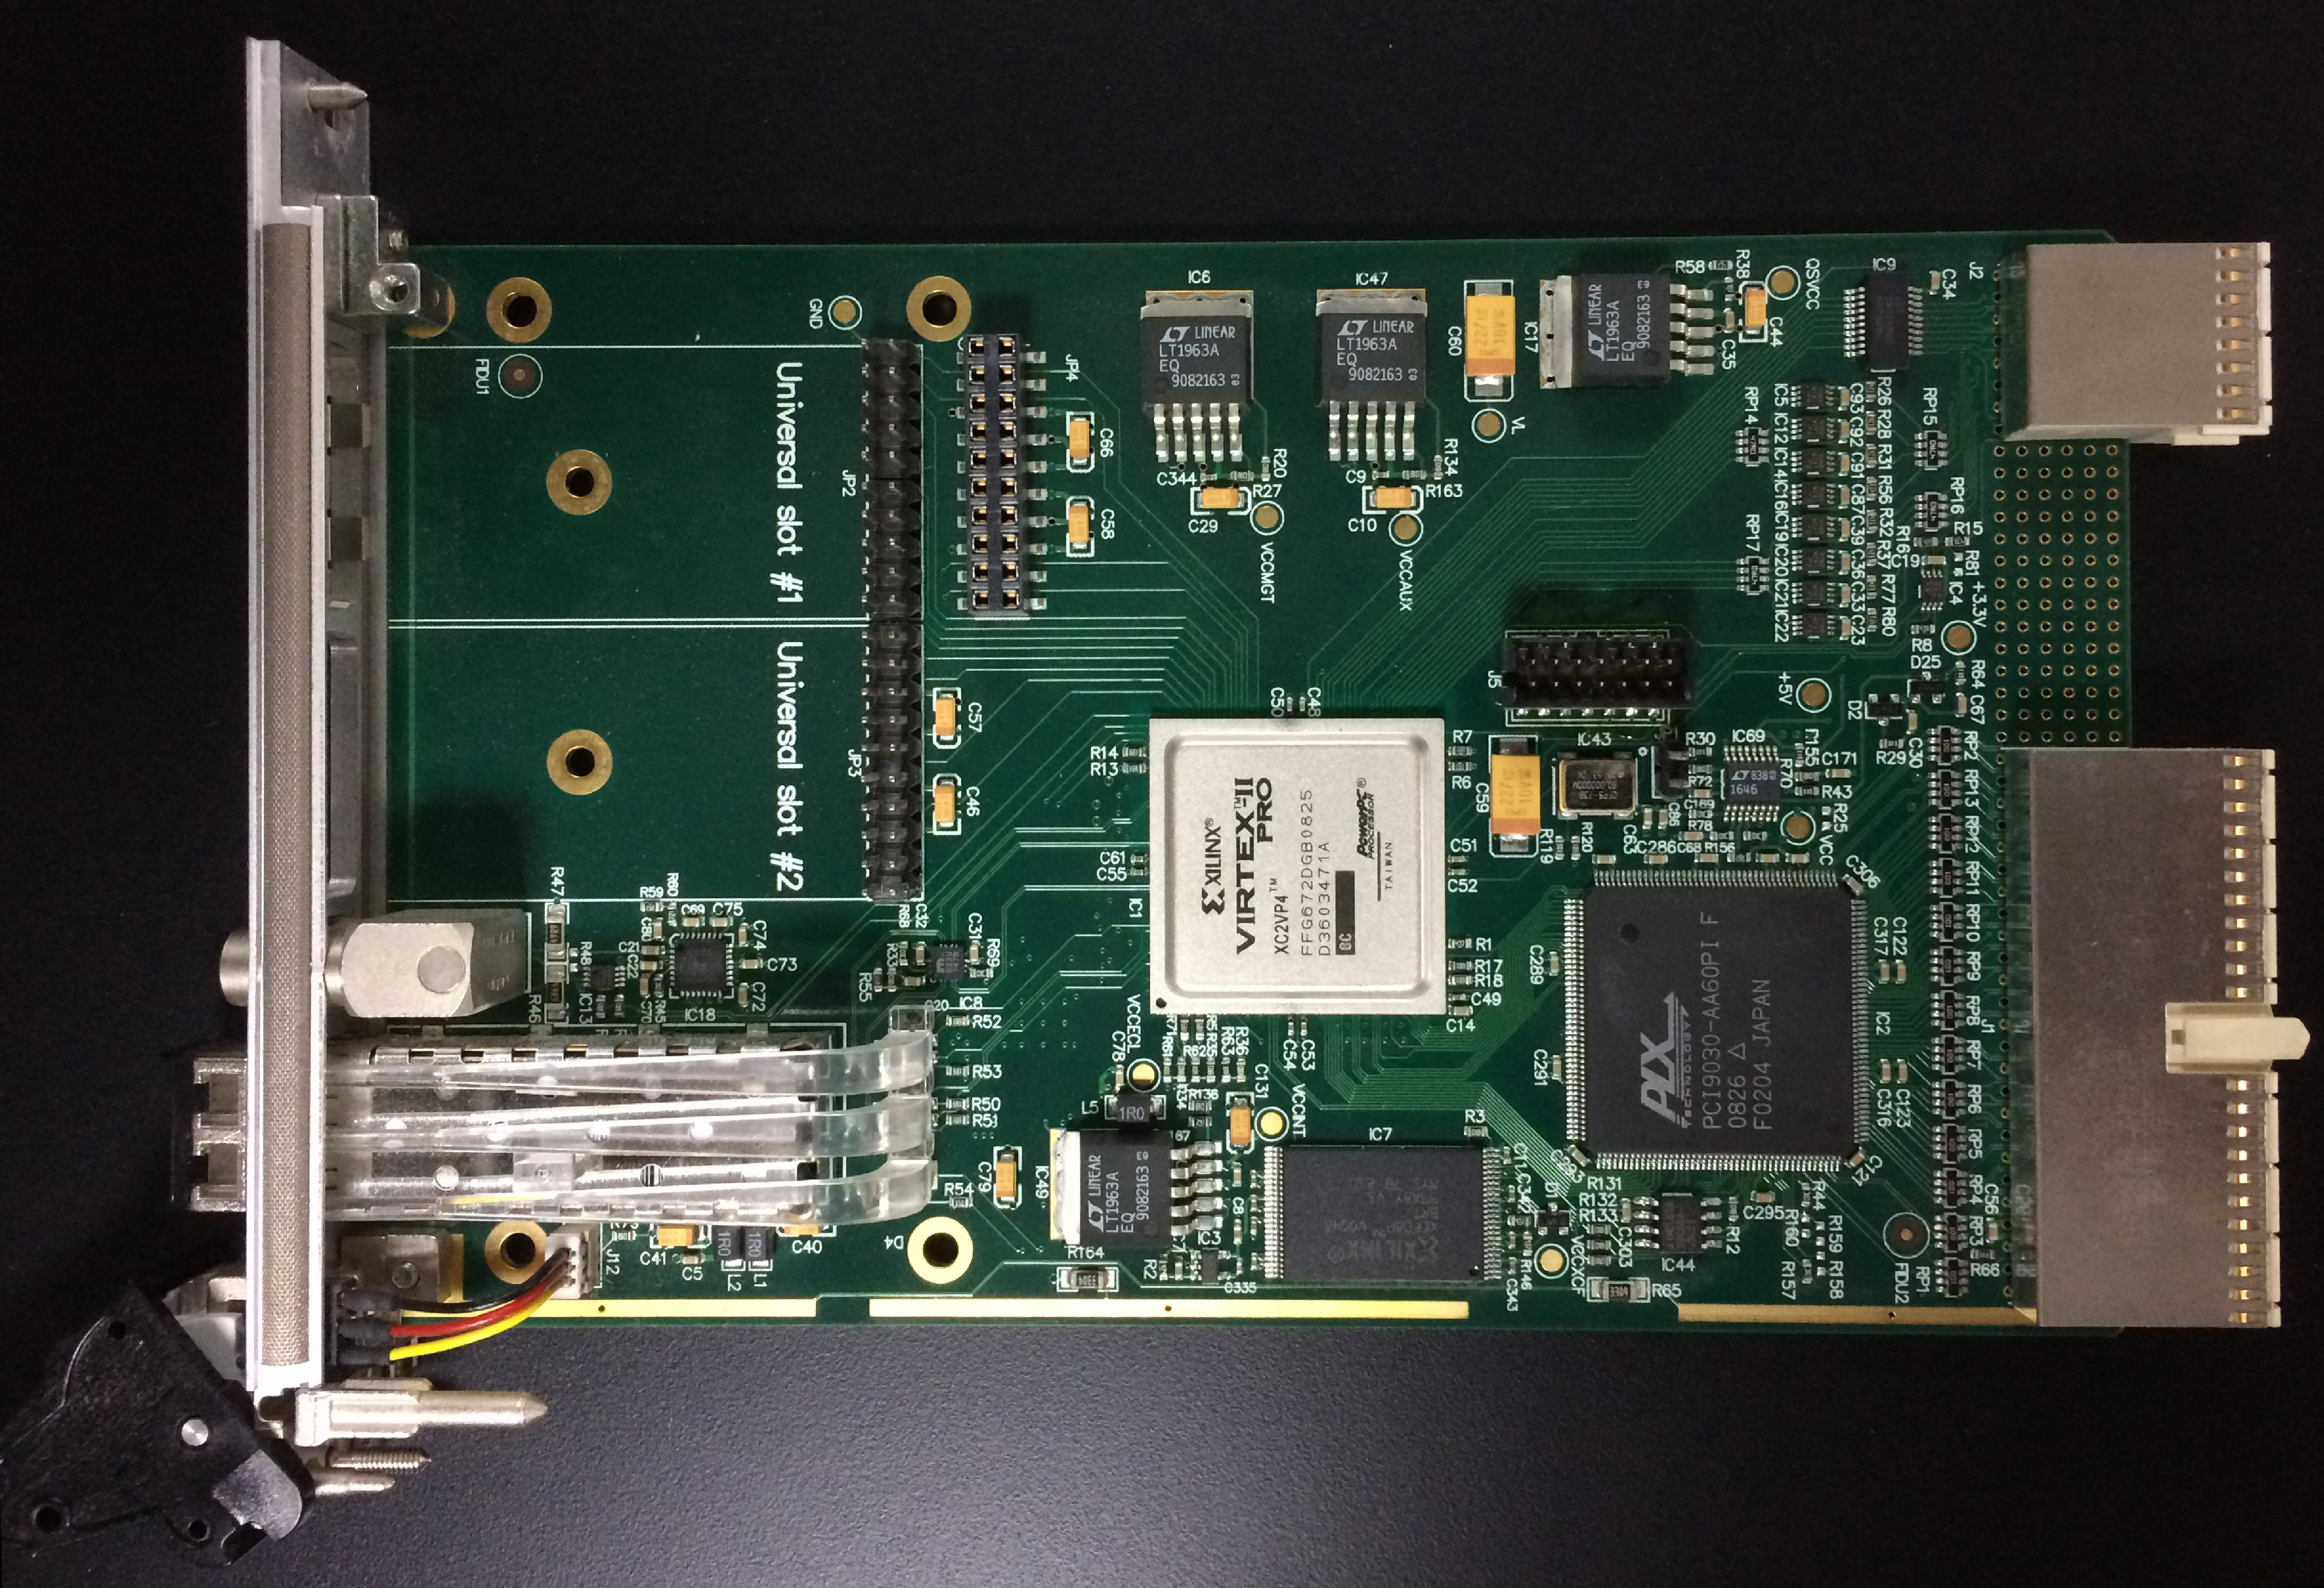
\includegraphics[width=0.99\textwidth]{./pictures/mrf_cpci_evg230}
  \caption{
    MRF cPCI-EVG-230.
  }
  \label{fig:cpci-evg230}
\end{figure}


The cPCI-EVG-230  has a SFP transceiver as an output to EVR/fan-out, one trigger input, one RF input and two universal I/O slots. Universal I/O modules are small mezzanines (25.6 mm x 50 mm) which are installed in these slots to provide different types of inputs, for example to trigger events.


\clearpage

\chapter{System Environment}
Before describing the engineering procedure for an E3 integration of the MRF cPCI-EVG-230 board, it is mandatory to have proper system environment that consists of specific hardware and software lists. Here we will show the hardware and software lists, their block diagrams, and their setup in the ICS lab at ESS. The information shown in this chapter is used in the ICS Lab at ESS.


\section{Hardware}
Table~\ref{table:hwlist} shows the hardware list and its environment. The form factor and version of EVR can be changeable. It is assumed that the proper working EVR is configured. Here, \texttt{TAG} is used as the prefix of the ICS internal inventory system in order to track it down.
\begin{table}[!hb]
  \centering
  \begin{tabular}{l|l|l}
    \toprule
    Hardware                 & Info                                         & Serial Number \\\midrule
    MRF cPCI-EVG-230         & \texttt{ICS TAG-805}                         & E283016       \\\midrule
    cPCI crate               & \texttt{ICS TAG-362}                         &               \\\midrule
    CPU                      & \texttt{ICS TAG-363}, hostname: icslab-ts01  & 43040574      \\\midrule
    MRF PCIe-EVR-300DC       & \texttt{ICS TAG-473}                         & M263057       \\\midrule
    MRF IFB-300              & \texttt{ICS TAG-352}                         & K472044       \\\midrule
    MRF Universal I/O module &                                              &               \\\midrule
    Adlink IPC               & \texttt{ICS TAG-837}, hostname: icslab-ipc01 & 93-41036-G10E \\\midrule
    Optical cables           & LC, Optical 850 nm                           &               \\\bottomrule
  \end{tabular}
  \caption[]{Hardware List.}
  \label{table:hwlist}
\end{table}


Figure~\ref{fig:hw-setup} shows the cPCI-EVG-230 in the crate, next to the CPU.
\begin{figure}[!b]
  \centering
  \includegraphics[width=0.8\textwidth]{./pictures/evgoncrate}
  \caption{Hardware Setup in the ICS lab.}
  \label{fig:hw-setup}
\end{figure}


\clearpage
\section{Software}
Table~\ref{table:swlist} shows the Software list and its environment. It is mandatory to check the kernel version, and the mrf kernel module version. Since the mrfioc2 is dependent upon devlib2 E3 internally, an end-user is unnecessary to check its version explicitly.
\begin{table}[!htb]
  \centering
  \begin{tabular}{l|l}
    \toprule
    Item               & Version Info.                                                      \\\midrule
    CentOS Linux       & \texttt{7.4.1708}                                                  \\\midrule
    Kernel             & \texttt{3.10.0-693.17.1.el7.x86\_64}                               \\\midrule
    mrf kernel module  & version : \texttt{1} / srcversion \texttt{A998B22F1425D7388F5F7A7} \\\midrule
    E3                 & \texttt{2.5.4}                                                     \\\midrule
    EPICS Base         & \texttt{3.15.5}                                                    \\\midrule
    mrfioc2            & E3 module ver. \texttt{2.2.0}                                      \\\midrule
    devLib2            & E3 module ver. \texttt{2.9.0}                                      \\\bottomrule
  \end{tabular}
  \caption[]{Software and its version information.}
  \label{table:swlist}
\end{table}

\section{EVG Firmware}
Table~\ref{table:fwinfo} shows EVG FPGA Firmware Version Register.

\begin{table}[!htb]
  \centering
  \begin{tabular}{p{0.3\linewidth}|c|l}
    \toprule
    EVG FPGA Firmware Version Register            & \multicolumn{2}{c}{\texttt{0x20000005}}             \\\midrule
    Board Type      & EVG                         &  \texttt{0x}\underline{\textbf{2}}\texttt{0000005}  \\\midrule
    Form Factor     & CompactPCI 3U               &  \texttt{0x2}\underline{\textbf{0}}\texttt{000005}  \\\midrule
    EVG Version ID  & 5                           &  \texttt{0x200000}\underline{\textbf{05}}           \\\bottomrule
  \end{tabular}
  \caption[]{EVG FPGA Firmware Version Register in Reference \citep[see][p32]{MRFEVENTGENERATOR}.}
  \label{table:fwinfo}
\end{table}


\clearpage
\chapter{Engineering Procedure}
This chapter provides the minimal information to configure the EVG board properly.

\section{System Installation}
Figure~\ref{fig:hw-setup} shows the glimpse of what system might be like in a Lab. The optical cable to EVR/fan-out is not shown.

\section{cPCI-EVG-230 Board Identification}

\subsection{Kernel Module}
It is essential to load the mrf kernel module and to check its information as follows:
\begin{lstlisting}[style=termstyle]
timinguser@icslab-ts01: ~$ modinfo mrf
filename:       /lib/modules/3.10.0-693.17.1.el7.x86_64/weak-updates/mrf.ko
author:         Michael Davidsaver <mdavidsaver@gmail.com>
version:        1
license:        GPL v2
rhelversion:    7.4
srcversion:     A998B22F1425D7388F5F7A7
alias:          pci:v000010EEd00007011sv00001A3Esd0000132Cbc*sc*i*
alias:          pci:v00001A3Ed0000152Csv00001A3Esd0000152Cbc*sc*i*
alias:          pci:v00001A3Ed0000252Csv00001A3Esd0000252Cbc*sc*i*
alias:          pci:v000010EEd00007011sv00001A3Esd0000172Cbc*sc*i*
alias:          pci:v00001204d0000EC30sv00001A3Esd0000172Cbc*sc*i*
alias:          pci:v000010B5d00009056sv00001A3Esd0000192Cbc*sc*i*
alias:          pci:v000010B5d00009030sv00001A3Esd000011E6bc*sc*i*
alias:          pci:v000010B5d00009030sv00001A3Esd000020E6bc*sc*i*
alias:          pci:v000010B5d00009030sv00001A3Esd000020DCbc*sc*i*
alias:          pci:v000010B5d00009030sv00001A3Esd000010E6bc*sc*i*
depends:        parport,uio
vermagic:       3.10.0-693.5.2.el7.x86_64 SMP mod_unload modversions
parm:           cable:Name of JTAG parallel port cable to emulate (charp)
parm:           interfaceversion:User space interface version (int)
parm:           use_msi:Use MSI if present (default 1, yes) (uint)
\end{lstlisting}

It is mandatory to check the access permission of an IOC user for the device file, e.g., \path{/dev/uio0} to allow the IOC process to open it. In case ones target system is NOT running \texttt{UDEV}, please consult the EVR user guide~\cite{EVR-USER-GUIDE}\footnote{Although this guide is intended for the EVR, the kernel module is the same for EVR and EVG}. And for building and loading the MRF kernel module and for changing the device file permission, please see Reference~\citep[see][p12,13]{EVR-USER-GUIDE}. It is inadvisable to change the file permission by using \texttt{chmod}.

\subsection{PCI Addressing}
Each PCI device is identified by a domain, a bus, a device, and a function number in Linux. Therefore, in order to initialize the MRF cPCI-EVG-230 board in E3, one needs the following information: a bus number, a device number, and a function number. These numbers are the parameters of a \texttt{mrmEvgSetupPCI} function.

One can use \texttt{lspci} to find them as follows:
\begin{lstlisting}[style=termstyle]
timinguser@icslab-ts01: ~$ lspci
...
16:0e.0 Signal processing controller: PLX Technology, Inc. PCI9030 32-bit 33MHz PCI <-> IOBus Bridge (rev 01)
...
timinguser@icslab-ts01: ~$ lspci -s 16:0e -vv
16:0e.0 Signal processing controller: PLX Technology, Inc. PCI9030 32-bit 33MHz PCI <-> IOBus Bridge (rev 01)
	Subsystem: Micro-Research Finland Oy CPCI Event Generator 230
	Control: I/O+ Mem+ BusMaster- SpecCycle- MemWINV- VGASnoop- ParErr- Stepping- SERR+ FastB2B- DisINTx-
	Status: Cap+ 66MHz- UDF- FastB2B+ ParErr- DEVSEL=medium >TAbort- <TAbort- <MAbort- >SERR- <PERR- INTx-
	Interrupt: pin A routed to IRQ 18
	Region 0: Memory at f0921000 (32-bit, non-prefetchable) [size=128]
	Region 2: Memory at f0910000 (32-bit, non-prefetchable) [size=64K]
	Capabilities: <access denied>
	Kernel driver in use: mrf-pci
	Kernel modules: mrf

\end{lstlisting}

And one should identify four number as follows:
\begin{lstlisting}[style=termstyle]
timinguser@icslab-ts01: ~$ lspci -s 16:0e -t
-+-[0000:16]---0e.0
 \-[0000:00]-

\end{lstlisting}
, where \texttt{-+-[0000:16]---0e.0} can be translated to \texttt{-+-}[domain:bus]\texttt{---}device.function. Thus in the above case, three numbers are shown in Table~\ref{table:pciidnumber}.\begin{table}[!htb]
  \centering
  \begin{tabular}{l|l}
    \toprule
    bus      & 0x16 \\\midrule
    device   & 0x0e \\\midrule
    function & 0x0 \\\bottomrule
  \end{tabular}
  \caption[]{MRF cPCI-EVG-230 Identification Numbers}
  \label{table:pciidnumber}
\end{table}


\clearpage
\section{EPICS IOC Setup under E3}
In order to start the EPICS IOC for the MRF cPCI-EVG-230 under E3, one should consider the following things: 1) the EPICS database file, and 2) the EPICS start-up script. The working directory, where an user can create, e.g., in the ICS Lab,
\begin{lstlisting}[style=termstyle, label={list:pwd}, caption={Working Directory in the ICS lab.} ]
/home/timinguser/ics_gitsrc/e3/e3-mrfioc2/cmds
\end{lstlisting}

\subsection{EPICS Database File}
The database file in E3 is located in the following location:
\begin{lstlisting}[style=termstyle]
/epics/modules/mrfioc2/2.2.0/R3.15.5/db/cpci-evg230-ess.db
\end{lstlisting}


\subsection{Start-Up Script}
Listing~\ref{list:emcpcievg230.cmd} shows the IOC start-up script which has the MRF cPCI-EVG-230 Identification Numbers, shown in Table~\ref{table:pciidnumber}. Note that the start-up script is located in the directory in Listing~\ref{list:pwd}.

\begin{lstlisting}[
    style=termstylenumber,
    label={list:emcpcievg230.cmd},
    caption={Start-up script \texttt{emcpcievg230.cmd}. Line \ref{pciid0} should be matched to Table~\ref{table:pciidnumber} as \texttt{mrmEvgSetupPCI(\$(DEV1), "bus:device.function")}.}
  ]
require mrfioc2, 2.2.0

epicsEnvSet("EPICS_CA_MAX_ARRAY_BYTES","10000000")

epicsEnvSet("IOC", "EMCPCIEVG230")
epicsEnvSet("DEV1", "EVG0")

epicsEnvSet("ESSEvtClockRate"  "88.0525") (*@\label{essfreq}@*)

mrmEvgSetupPCI($(DEV1), "16:0e.0") (*@\label{pciid0}@*)
dbLoadRecords("cpci-evg230-ess.db",  "SYS=$(IOC), D=$(DEV1), EVG=$(DEV1), FEVT=$(ESSEvtClockRate), FRF=$(ESSEvtClockRate), FDIV=1")

iocInit()
\end{lstlisting}

\subsection{EPICS IOC}
All the EPICS parameters should be run from an E3 session. To start E3, type:
\begin{lstlisting}[style=termstyle]
[timinguser@icslab-ts01 ~]$ source source /home/timinguser/ics_gitsrc/e3/e3-env/setE3Env.bash
\end{lstlisting}
All the IOCs and related EPICS commands (caget, caput, camonitor, etc.) should be run from an E3 session.

Under E3, the EPICS IOC can be started via the command \texttt{iocsh.bash emcpcievg230.cmd}. The output should look like as follows:

\begin{lstlisting}[style=termstyle]
[timinguser@icslab-ts01 cmds]$ iocsh.bash emcpcievg230.cmd
#
# Start at "2018-W29-Jul19-1556-18-CEST"
#
# Version information:
# European Spallation Source ERIC : iocsh.bash (v0.2-9d66ded.PID-1051)
## can you see this?
#
# HOSTDISPLAY=""
# WINDOWID=""
# PWD="/home/timinguser/ics_gitsrc/e3/e3-mrfioc2/cmds"
# USER="timinguser"
# LOGNAME="timinguser"
# EPICS_HOST_ARCH="linux-x86_64"
# EPICS_BASE="/epics/bases/base-3.15.5"
# EPICS_LOCATION="/epics/bases"
# EPICS="/epics/bases"
# EPICS_MODULES="/epics/modules"
# REQUIRE="require"
# REQUIRE_VERSION="2.5.4"
# REQUIRE_BIN="/epics/modules/require/2.5.4/bin"
# REQUIRE_LIB="/epics/modules/require/2.5.4/R3.15.5/lib"
# REQUIRE_DBD="/epics/modules/require/2.5.4/R3.15.5/dbd"
# EPICS_CA_AUTO_ADDR_LIST="yes"
# EPICS_CA_ADDR_LIST=""
# PATH="/epics/modules/require/2.5.4/bin:/epics/bases/base-3.15.5/bin/linux-x86_64:/usr/local/bin:/usr/bin:/bin:/usr/local/games:/usr/games:/sbin:/home/timinguser/bin:/opt/etherlab/bin:/opt/etherlab/sbin"
# LD_LIBRARY_PATH="/epics/bases/base-3.15.5/lib/linux-x86_64:/epics/modules/require/2.5.4/R3.15.5/lib/linux-x86_64:/usr/local/lib:/home/timinguser/lib:/opt/etherlab/lib"
#
# Please Use Version and other environment variables
# in order to report or debug this shell
#
# Loading the mandatory require module ...
#
dlload /epics/modules/require/2.5.4/R3.15.5/lib/linux-x86_64/librequire.so
dbLoadDatabase /epics/modules/require/2.5.4/R3.15.5/dbd/require.dbd
require_registerRecordDeviceDriver
Loading module info records for require
#
#
< "emcpcievg230.cmd"
require mrfioc2, 2.2.0
Module mrfioc2 version 2.2.0 found in /epics/modules/mrfioc2/2.2.0/
Module mrfioc2 depends on devlib2 2.9+
Module devlib2 version 2.9.0 found in /epics/modules/devlib2/2.9.0/
Loading library /epics/modules/devlib2/2.9.0/R3.15.5/lib/linux-x86_64/libdevlib2.so
Loaded devlib2 version 2.9.0
Loading dbd file /epics/modules/devlib2/2.9.0/R3.15.5/dbd/devlib2.dbd
Calling function devlib2_registerRecordDeviceDriver
Loading module info records for devlib2
Loading library /epics/modules/mrfioc2/2.2.0/R3.15.5/lib/linux-x86_64/libmrfioc2.so
Loaded mrfioc2 version 2.2.0
Loading dbd file /epics/modules/mrfioc2/2.2.0/R3.15.5/dbd/mrfioc2.dbd
Calling function mrfioc2_registerRecordDeviceDriver
Loading module info records for mrfioc2
epicsEnvSet("EPICS_CA_MAX_ARRAY_BYTES","10000000")
epicsEnvSet("IOC", "EMCPCIEVG230")
epicsEnvSet("DEV1", "EVG0")
epicsEnvSet("ESSEvtClockRate"  "88.0525")
mrmEvgSetupPCI(EVG0, "16:0e.0")
Notice: devPCIFindSpec() expect B:D.F in hex
Device EVG0  22:14.0
Using IRQ 18
FPGA version: 20000005
Firmware version >= 3 is recommended, please consider upgrading
PCI interrupt connected!
dbLoadRecords("cpci-evg230-ess.db",  "SYS=EMCPCIEVG230, D=EVG0, EVG=EVG0, FEVT=88.0525, FRF=88.0525, FDIV=1")
macLib: macro PINITSEQ is undefined (expanding string # $(PINITSEQ,undefined)Cont-FOut_
)
Warning: 'cpci-evg230-ess.db' line 3602 has undefined macros
macLib: macro PINITSEQ is undefined (expanding string # $(PINITSEQ,undefined)Cont-FOut_
)
Warning: 'cpci-evg230-ess.db' line 3706 has undefined macros
macLib: macro PINITSEQ is undefined (expanding string # $(PINITSEQ,undefined)Cont-FOut_
)
Warning: 'cpci-evg230-ess.db' line 3810 has undefined macros
iocInit()
Starting iocInit
############################################################################
## EPICS R3.15.5-EEE-3.15.5-patch
## EPICS Base built Jan  5 2018
############################################################################
require: record EMCPCIEVG230:MODULES not found
require: record EMCPCIEVG230:VERSIONS not found
require: record EMCPCIEVG230:MOD_VER not found
iocRun: All initialization complete
epicsEnvSet IOCSH_PS1 "9d66ded.icslab-ts01.1067 > "
epicsEnvShow T_A
T_A=linux-x86_64
epicsEnvShow EPICS_HOST_ARCH
EPICS_HOST_ARCH=linux-x86_64
9d66ded.icslab-ts01.1067 >
\end{lstlisting}

In addition, the PCI information is available within the running IOC via \texttt{devPCIShow} as follows:
\begin{lstlisting}
9d66ded.icslab-ts01.2759 > devPCIShow
\end{lstlisting}
Look for the line with your configuration information, in our case is:
\begin{lstlisting}
PCI 0000:16:0e.0 IRQ 18
  vendor:device 10b5:9030 rev 00
\end{lstlisting}
Where the vendor id 10b5 is PLX Technology INC.
And show the PCI information with (the second parameter is the verbosity level):
\begin{lstlisting}
9d66ded.icslab-ts01.2759 > devPCIShow 9 0x10b5
...
PCI 0000:16:0e.0 IRQ 18
  vendor:device 10b5:9030 rev 00
  subved:subdev 1a3e:20e6
  class 118000 generic signal processing controller
  driver mrf-pci
  BAR 0 32-bit MMIO    128 B
  BAR 2 32-bit MMIO     64 kB
...
\end{lstlisting}

\newpage
\chapter{System In-Situ Configuration}
This chapter how to configure the EVG according to one's needs.
\begin{table}[!htb]
  \centering
  \begin{tabular}{c|p{0.4\linewidth}|p{0.42\linewidth}}
    \toprule
    Step & Goal                                            & Info.                                                 \\\midrule
    0    & Select the event frequency                      & Link clock                                            \\\midrule
    1    & Emit a software triggered event                 & SW event emission                                     \\\midrule
    2    & Emit a periodic event                           & Multiplexed counters                                  \\\midrule
    3    & Emit a sequence                                 & Create a sequence, commit and emit it                 \\\midrule
    4    & Emit an event triggered from an external source & Trigger the event emission from an external device    \\\bottomrule
  \end{tabular}
  \caption[]{System In-Situ Verification Procedure}
  \label{table:checklist}
\end{table}


\section{Step 0 : Select the event frequency}
One can check and select the event frequency with these commands after loading the E3 environment. Short comments on each command or a series of commands are shown before the corresponding command.
\begin{lstlisting}[style=termstyle]
#
# Check the event frequency; here the ESS frequency is shown
#
timinguser@icslab-ts01: ~$ caget EMCPCIEVG230-EVG0:EvtClk-Frequency-RB
EMCPCIEVG230-EVG0:EvtClk-Frequency-RB 88.0519
\end{lstlisting}
The ESS frequency (88.0525 MHz) was selected in line \ref{essfreq} of the startup script in Listing~\ref{list:emcpcievg230.cmd}. A slightly different frequency is shown because of the capabilities of the internal frequency synthesizer. In operations the EVG will get the event frequency from the master RF oscillator.
\begin{lstlisting}[style=termstyle]
#
# Change the event frequency to 100 MHz
#
timinguser@icslab-ts01: ~$ caput EMCPCIEVG230-EVG0:EvtClk-FracSynFreq-SP 100
Old : EMCPCIEVG230-EVG0:EvtClk-FracSynFreq-SP 88.0525
New : EMCPCIEVG230-EVG0:EvtClk-FracSynFreq-SP 100
#
# Check the new event frequency
#
timinguser@icslab-ts01: ~$ caget EMCPCIEVG230-EVG0:EvtClk-Frequency-RB
EMCPCIEVG230-EVG0:EvtClk-Frequency-RB 100
#
# Revert back to the ESS event frequency and check it
#
timinguser@icslab-ts01: ~$ caput EMCPCIEVG230-EVG0:EvtClk-FracSynFreq-SP 88.0525
Old : EMCPCIEVG230-EVG0:EvtClk-FracSynFreq-SP 100
New : EMCPCIEVG230-EVG0:EvtClk-FracSynFreq-SP 88.0525
timinguser@icslab-ts01: ~$ caget EMCPCIEVG230-EVG0:EvtClk-Frequency-RB
EMCPCIEVG230-EVG0:EvtClk-Frequency-RB 88.0519
\end{lstlisting}

\section{Step 1 : Emit a software triggered event}
In this step the connection to an EVR will be checked. In addition to the EVG, the EVR (correctly installed) and an optical cable between both are needed. In this example the EVR is installed in a different crate than the EVG. The start-up script file for the EVG is the same as shown in Listing~\ref{list:emcpcievg230.cmd}.

Following are the steps necessary to emit the event and check that it is received in the EVR. Short comments on each command or a series of commands are shown before the corresponding command.

\begin{lstlisting}[style=termstyle]
#
# Monitor the arrival of event 10 on the EVR
#
iocuser@icslab-ipc01: ~$ camonitor EMCPCIEVG230-EVR0:EvtACnt-I
EMCPCIEVG230-EVR0:EvtACnt-I    <undefined> 0 UDF INVALID
#
# Send the software event 10 from the EVG
#
timinguser@icslab-ts01: ~$ caput EMCPCIEVG230-EVG0:SoftEvt-EvtCode-SP 10
Old : EMCPCIEVG230-EVG0:SoftEvt-EvtCode-SP 0
New : EMCPCIEVG230-EVG0:SoftEvt-EvtCode-SP 10
#
# Check that the EVR has received the event
#
iocuser@icslab-ipc01: ~$ camonitor EMCPCIEVG230-EVR0:EvtACnt-I
EMCPCIEVG230-EVR0:EvtACnt-I    <undefined> 0 UDF INVALID
EMCPCIEVG230-EVR0:EvtACnt-I    <undefined> 1
#
# One can repeat this process several times
#
timinguser@icslab-ts01: ~$ caput EMCPCIEVG230-EVG0:SoftEvt-EvtCode-SP 10
Old : EMCPCIEVG230-EVG0:SoftEvt-EvtCode-SP 10
New : EMCPCIEVG230-EVG0:SoftEvt-EvtCode-SP 10
timinguser@icslab-ts01: ~$ caput EMCPCIEVG230-EVG0:SoftEvt-EvtCode-SP 10
Old : EMCPCIEVG230-EVG0:SoftEvt-EvtCode-SP 10
New : EMCPCIEVG230-EVG0:SoftEvt-EvtCode-SP 10
timinguser@icslab-ts01: ~$ caput EMCPCIEVG230-EVG0:SoftEvt-EvtCode-SP 10
Old : EMCPCIEVG230-EVG0:SoftEvt-EvtCode-SP 10
New : EMCPCIEVG230-EVG0:SoftEvt-EvtCode-SP 10
#
# Which can be seen on the EVR
#
EMCPCIEVG230-EVR0:EvtACnt-I    <undefined> 2
EMCPCIEVG230-EVR0:EvtACnt-I    <undefined> 3
EMCPCIEVG230-EVR0:EvtACnt-I    <undefined> 4
\end{lstlisting}

\subsection{Step 1.1 : Configure the EVG to send the timestamp}
Only one more line is needed in the EVG startup script to send the timestamp from the EVG to the EVRs. One must add the following line after \path{iocInit()} in Listing~\ref{list:emcpcievg230.cmd}:
\begin{lstlisting}[style=termstyle]
dbpf "$(IOC)-$(DEV1):1ppsInp-Sel" "Sys Clk"
\end{lstlisting}

In this case the camonitor of the event will show its correct timestamp:
\begin{lstlisting}[style=termstyle]
#
# Send the event from the EVG
#
timinguser@icslab-ts01: ~$ caput EMCPCIEVG230-EVG0:SoftEvt-EvtCode-SP 10
Old : EMCPCIEVG230-EVG0:SoftEvt-EvtCode-SP 0
New : EMCPCIEVG230-EVG0:SoftEvt-EvtCode-SP 10
timinguser@icslab-ts01: ~$ caput EMCPCIEVG230-EVG0:SoftEvt-EvtCode-SP 10
Old : EMCPCIEVG230-EVG0:SoftEvt-EvtCode-SP 10
New : EMCPCIEVG230-EVG0:SoftEvt-EvtCode-SP 10
timinguser@icslab-ts01: ~$ caput EMCPCIEVG230-EVG0:SoftEvt-EvtCode-SP 10
Old : EMCPCIEVG230-EVG0:SoftEvt-EvtCode-SP 10
New : EMCPCIEVG230-EVG0:SoftEvt-EvtCode-SP 10
timinguser@icslab-ts01: ~$ caput EMCPCIEVG230-EVG0:SoftEvt-EvtCode-SP 10
Old : EMCPCIEVG230-EVG0:SoftEvt-EvtCode-SP 10
New : EMCPCIEVG230-EVG0:SoftEvt-EvtCode-SP 10
#
# Monitor the event in the EVR
#
iocuser@icslab-ipc01: ~$ camonitor EMCPCIEVG230-EVR0:EvtACnt-I
EMCPCIEVG230-EVR0:EvtACnt-I    <undefined> 0 UDF INVALID
EMCPCIEVG230-EVR0:EvtACnt-I    2018-07-20 11:36:12.144397 1
EMCPCIEVG230-EVR0:EvtACnt-I    2018-07-20 11:36:13.018189 2
EMCPCIEVG230-EVR0:EvtACnt-I    2018-07-20 11:36:13.468005 3
EMCPCIEVG230-EVR0:EvtACnt-I    2018-07-20 11:36:13.941891 4
\end{lstlisting}


\section{Step 2 : Emit a periodic event}
The EVG can be set to emit periodically an event by using a multiplexed counter (Mxc). Short comments on each command or a series of commands are shown before the corresponding command. In this example the Mxc7 is used to create the heartbeat event (event number 122) at a frequency of 1 Hz.
\begin{lstlisting}[style=termstyle]
#
# Set up the Mxc7 frequency to 1 Hz, by dividing the event clock (88.0525 MHz) by the integer number set in this record (88.0525MHz/88052500=1Hz)
#
timinguser@icslab-ts01: ~$ caput EMCPCIEVG230-EVG0:Mxc7-Prescaler-SP 88052500
Old : EMCPCIEVG230-EVG0:Mxc7-Prescaler-SP 124920
New : EMCPCIEVG230-EVG0:Mxc7-Prescaler-SP 88052500
#
# Set the trigger event source 7 event code to 122
#
timinguser@icslab-ts01: ~$ caput EMCPCIEVG230-EVG0:TrigEvt7-EvtCode-SP 122
Old : EMCPCIEVG230-EVG0:TrigEvt7-EvtCode-SP 0
New : EMCPCIEVG230-EVG0:TrigEvt7-EvtCode-SP 122
#
# Set the trigger event source 7 to trigger on the tick of Mxc7 (map the trigger event source to the Mxc7)
#
timinguser@icslab-ts01: ~$ caput EMCPCIEVG230-EVG0:TrigEvt7-TrigSrc-Sel "Mxc7"
Old : EMCPCIEVG230-EVG0:TrigEvt7-TrigSrc-Sel Off
New : EMCPCIEVG230-EVG0:TrigEvt7-TrigSrc-Sel Mxc7
\end{lstlisting}
One can check the arrival of event 122 (or heartbeat event) in the EVR by monitoring the link timeout record \path{$(SYS)-$(D):Cnt-LinkTimo-I}. Before the event is set, this record increases its value by 1 every 1.6 s approximately. When the heartbeat event is being received at 1 Hz (or actually at any rate faster than 1.6 s) this record does not increase.

The heartbeat event, or any other event at any desired frequency, can be set automatically at startup by including in the startup script the same commands after \path{iocInit()} in Listing~\ref{list:emcpcievg230.cmd}, and replacing \path{caput} by \path{dbpf}.


\section{Step 3 : Emit a sequence}
In this section it is shown how to configure a sequencer to emit a sequence of events. Short comments on each command or a series of commands are shown before the corresponding command.
\begin{lstlisting}[style=termstyle]
#
# Attach the soft sequence to a specific hardware sequence
#
timinguser@icslab-ts01 ~]$ caput EMCPCIEVG230-EVG0:SoftSeq0-Unload-Cmd 1
Old : EMCPCIEVG230-EVG0:SoftSeq0-Unload-Cmd 0
New : EMCPCIEVG230-EVG0:SoftSeq0-Unload-Cmd 1
[timinguser@icslab-ts01 ~]$ caput EMCPCIEVG230-EVG0:SoftSeq0-Load-Cmd 1
Old : EMCPCIEVG230-EVG0:SoftSeq0-Load-Cmd 0
New : EMCPCIEVG230-EVG0:SoftSeq0-Load-Cmd 1
#
# Set the engineering units (microseconds) for the delay of the events in the sequence (sequence timestamps)
#
[timinguser@icslab-ts01 ~]$ caput EMCPCIEVG230-EVG0:SoftSeq0-TsResolution-Sel "uSec"
Old : EMCPCIEVG230-EVG0:SoftSeq0-TsResolution-Sel Ticks
New : EMCPCIEVG230-EVG0:SoftSeq0-TsResolution-Sel uSec
#
# Set the trigger source for the sequence as software and enable it
#
[timinguser@icslab-ts01 ~]$ caput EMCPCIEVG230-EVG0:SoftSeq0-TrigSrc-Sel "Software"
Old : EMCPCIEVG230-EVG0:SoftSeq0-TrigSrc-Sel None
New : EMCPCIEVG230-EVG0:SoftSeq0-TrigSrc-Sel Software
[timinguser@icslab-ts01 ~]$ caput EMCPCIEVG230-EVG0:SoftSeq0-Enable-Cmd 1
Old : EMCPCIEVG230-EVG0:SoftSeq0-Enable-Cmd 0
New : EMCPCIEVG230-EVG0:SoftSeq0-Enable-Cmd 1
#
# Set the runmode to normal, so that the sequencer re-arms after it finishes running
#
[timinguser@icslab-ts01 ~]$ caput EMCPCIEVG230-EVG0:SoftSeq0-RunMode-Sel "Normal"
Old : EMCPCIEVG230-EVG0:SoftSeq0-RunMode-Sel Single
New : EMCPCIEVG230-EVG0:SoftSeq0-RunMode-Sel Normal
#
# Set up the sequence content, events and timestamps
# Event 127 is always needed at the end, it is the end-of-sequence event and stops the sequencer
# The timestamps are specified in microseconds, as set before
# In this example, events 10, 11 and 12 are issued 1 s, 2 s and 3 s after triggering the sequencer
#
[timinguser@icslab-ts01 ~]$ caput -a EMCPCIEVG230-EVG0:SoftSeq0-EvtCode-SP 4 10 11 12 127
Old : EMCPCIEVG230-EVG0:SoftSeq0-EvtCode-SP 2047 3 0 0 0 [...]
New : EMCPCIEVG230-EVG0:SoftSeq0-EvtCode-SP 2047 10 11 12 127 0 0 0 [...]
[timinguser@icslab-ts01 ~]$ caput -a EMCPCIEVG230-EVG0:SoftSeq0-Timestamp-SP 4 1000000 2000000 3000000 3000001
Old : EMCPCIEVG230-EVG0:SoftSeq0-Timestamp-SP 2047 0 0 0 [...]
New : EMCPCIEVG230-EVG0:SoftSeq0-Timestamp-SP 2047 1e+06 2e+06 3e+06 3e+06 0 0 0 [...]
#
# Commit the sequence to hardware
#
[timinguser@icslab-ts01 ~]$ caput EMCPCIEVG230-EVG0:SoftSeq0-Commit-Cmd 1
Old : EMCPCIEVG230-EVG0:SoftSeq0-Commit-Cmd Commit
New : EMCPCIEVG230-EVG0:SoftSeq0-Commit-Cmd Commit
#
# On the EVR, monitor the reception of the events
#
[iocuser@icslab-ipc01 ~]$ camonitor EMCPCIEVG230-EVR0:EvtACnt-I EMCPCIEVG230-EVR0:EvtBCnt-I EMCPCIEVG230-EVR0:EvtCCnt-I
EMCPCIEVG230-EVR0:EvtACnt-I    <undefined> 0 UDF INVALID
EMCPCIEVG230-EVR0:EvtBCnt-I    <undefined> 0 UDF INVALID
EMCPCIEVG230-EVR0:EvtCCnt-I    <undefined> 0 UDF INVALID
#
# On the EVG host, trigger the sequence
#
[timinguser@icslab-ts01 ~]$ caput EMCPCIEVG230-EVG0:SoftSeq0-SoftTrig-Cmd 1
Old : EMCPCIEVG230-EVG0:SoftSeq0-SoftTrig-Cmd 0
New : EMCPCIEVG230-EVG0:SoftSeq0-SoftTrig-Cmd 1
#
# The EVR will receive these events
#
EMCPCIEVG230-EVR0:EvtACnt-I    2018-07-23 10:26:19.089541 1
EMCPCIEVG230-EVR0:EvtBCnt-I    2018-07-23 10:26:20.089570 1
EMCPCIEVG230-EVR0:EvtCCnt-I    2018-07-23 10:26:21.089623 1
#
# This can be repeated
#
[timinguser@icslab-ts01 ~]$ caput EMCPCIEVG230-EVG0:SoftSeq0-SoftTrig-Cmd 1
Old : EMCPCIEVG230-EVG0:SoftSeq0-SoftTrig-Cmd 1
New : EMCPCIEVG230-EVG0:SoftSeq0-SoftTrig-Cmd 1
[timinguser@icslab-ts01 ~]$ caput EMCPCIEVG230-EVG0:SoftSeq0-SoftTrig-Cmd 1
Old : EMCPCIEVG230-EVG0:SoftSeq0-SoftTrig-Cmd 1
New : EMCPCIEVG230-EVG0:SoftSeq0-SoftTrig-Cmd 1
#
# EVR output
#
EMCPCIEVG230-EVR0:EvtACnt-I    2018-07-23 10:26:44.068009 2
EMCPCIEVG230-EVR0:EvtBCnt-I    2018-07-23 10:26:45.068040 2
EMCPCIEVG230-EVR0:EvtCCnt-I    2018-07-23 10:26:46.068068 2
EMCPCIEVG230-EVR0:EvtACnt-I    2018-07-23 10:26:50.579669 3
EMCPCIEVG230-EVR0:EvtBCnt-I    2018-07-23 10:26:51.579688 3
EMCPCIEVG230-EVR0:EvtCCnt-I    2018-07-23 10:26:52.579727 3
\end{lstlisting}

It is possible to run the sequencer automatically triggered by a Mxc; for example, for Mxc0:
\begin{lstlisting}
[timinguser@icslab-ts01 ~]$ caput EMCPCIEVG230-EVG0:SoftSeq0-TrigSrc-Sel "Mxc0"
\end{lstlisting}

All the previous commands, except the set up of the sequence content (the event and timestamp lists) and the commit command which has to be run at the end of the configuration including the sequence content, can be set automatically at startup by including in the startup script the same commands after \path{iocInit()} in Listing~\ref{list:emcpcievg230.cmd}, and replacing \path{caput} by \path{dbpf}.

It is also possible to set up the sequence content automatically by creating a file with the commands to configure the sequence contents and the commit command (with \path{caput}, not \path{dbpf}). This file looks like Listing~\ref{list:configuresequence.sh} and should be in the same directory as the startup script.
\begin{lstlisting}[
    style=termstyle,
    label={list:configuresequence.sh},
    caption={Configure the sequence contents and commit commands file \texttt{configuresequence.sh}.}
  ]
caput -a EMCPCIEVG230-EVG0:SoftSeq0-EvtCode-SP 4 10 11 12 127

caput -a EMCPCIEVG230-EVG0:SoftSeq0-Timestamp-SP 4 1000000 2000000 3000000 3000001

caput EMCPCIEVG230-EVG0:SoftSeq0-Commit-Cmd 1
\end{lstlisting}

This file should be called from the IOC shell including the following line after \path{iocInit()} and all the sequencer configuration lines:
\begin{lstlisting}
system("/bin/sh ./configuresequence.sh")
\end{lstlisting}


\section{Step 4 : Emit an event triggered from an external source}
In this step the event emission is triggered from an external input. It will be necessary to install an I/O module to the cPCI-EVG-230 board. The start-up script file for the EVG is the same one as shown in Listing~\ref{list:emcpcievg230.cmd}.

Short comments on each command or a series of commands are shown before the corresponding command.

\begin{lstlisting}[style=termstyle]
#
# Set event code 10 to be emitted when trigger source 1 is triggered
#
[timinguser@icslab-ts01 ~]$ caput EMCPCIEVG230-EVG0:TrigEvt1-EvtCode-SP 10
Old : EMCPCIEVG230-EVG0:TrigEvt1-EvtCode-SP 0
New : EMCPCIEVG230-EVG0:TrigEvt1-EvtCode-SP 10
#
# Map universal input 0 to trigger source 1
#
[timinguser@icslab-ts01 ~]$ caput EMCPCIEVG230-EVG0:TrigEvt1-TrigSrc-Sel "Univ0"
Old : EMCPCIEVG230-EVG0:TrigEvt1-TrigSrc-Sel Off
New : EMCPCIEVG230-EVG0:TrigEvt1-TrigSrc-Sel Univ0
#
# Trigger the input with your external device
# It is possible to check the reception of the event in an EVR, as shown before
#
\end{lstlisting}
As always this can be included in the startup script.


\newpage
\chapter{Use case: generate 14 Hz with a sequencer}
The startup script for an IOC that automatically generates a 14 Hz signal using a sequencer is shown in Listing~\ref{list:emcpcievg230_14Hz.cmd}. In the same directory the file shown in Listing~\ref{list:configuresequence_14Hz.sh} should be present.
\begin{lstlisting}[
    style=termstyle,
    label={list:emcpcievg230_14Hz.cmd},
    caption={Start-up script \texttt{emcpcievg230\_14Hz.cmd}.}
  ]
#
# This the full setup for the Timing System with E3.
#

require mrfioc2, 2.2.0

epicsEnvSet("EPICS_CA_MAX_ARRAY_BYTES","10000000")

epicsEnvSet("IOC", "EMCPCIEVG230")
epicsEnvSet("DEV1", "EVG0")
epicsEnvSet("PCIADDR", "16:0e.0")

epicsEnvSet("MainEvtCODE" "14")
epicsEnvSet("HeartBeatEvtCODE"   "122")
epicsEnvSet("ESSEvtClockRate"  "88.0525")

mrmEvgSetupPCI($(DEV1), $(PCIADDR))
dbLoadRecords("cpci-evg230-ess.db",  "SYS=$(IOC), D=$(DEV1), EVG=$(DEV1), FEVT=$(ESSEvtClockRate), FRF=$(ESSEvtClockRate), FDIV=1")

iocInit()

dbpf "$(IOC)-$(DEV1):1ppsInp-Sel" "Sys Clk"

# Master Event Rate 14 Hz
dbpf $(IOC)-$(DEV1):Mxc0-Prescaler-SP 6289464

# Setup of sequencer
dbpf $(IOC)-$(DEV1):SoftSeq0-RunMode-Sel "Normal"
dbpf $(IOC)-$(DEV1):SoftSeq0-TrigSrc-Sel "Mxc0"
dbpf $(IOC)-$(DEV1):SoftSeq0-TsResolution-Sel "uSec"
dbpf $(IOC)-$(DEV1):SoftSeq0-Load-Cmd 1
dbpf $(IOC)-$(DEV1):SoftSeq0-Enable-Cmd 1

# Load the sequence
system("/bin/sh ./configure_sequence.sh $(IOC) $(DEV1)")

# Heart Beat 1 Hz
dbpf $(IOC)-$(DEV1):Mxc7-Prescaler-SP 88052500
dbpf $(IOC)-$(DEV1):TrigEvt7-EvtCode-SP $(HeartBeatEvtCODE)
dbpf $(IOC)-$(DEV1):TrigEvt7-TrigSrc-Sel "Mxc7"

dbpf $(IOC)-$(DEV1):SyncTimestamp-Cmd 1
\end{lstlisting}

\begin{lstlisting}[
    style=termstyle,
    label={list:configuresequence_14Hz.sh},
    caption={Sequencer content script \texttt{configuresequence\_14Hz.sh}.}
  ]
# Bash script to configure the EVG/EVR sequencer
# All values in us

# Event code 14 (14 Hz), 127 is the end of sequence
caput -a $1-$2:SoftSeq0-EvtCode-SP 2 14 127

# Defining time at which the event codes are sent in us
caput -a $1-$2:SoftSeq0-Timestamp-SP 2 0 1

# Commit the sequence to HW
caput $1-$2:SoftSeq0-Commit-Cmd 1
\end{lstlisting}

\clearpage
\backmatter
%\bibliographystyle{unsrt}
%\bibliographystyle{plainnat}
%\bibliographystyle{abbrvnat}
\bibliographystyle{unsrtnat}
%\bibliographystyle{chicago}
\bibliography{./ess_refs}

\end{document}



%% The output of \verb|lspci| for the PCIe-EVR-300 is:
%% \begin{lstlisting}
%% $ lspci -s 05:00 -vv
%% 05:00.0 Signal processing controller: Lattice Semiconductor Corporation Device
%%         ec30 (rev 01)
%%     Subsystem: Device 1a3e:172c
%%     Control: I/O+ Mem+ BusMaster+ SpecCycle- MemWINV- VGASnoop- ParErr-
%%         Stepping- SERR- FastB2B- DisINTx-
%%     Status: Cap+ 66MHz- UDF- FastB2B- ParErr- DEVSEL=fast >TAbort- <TAbort-
%%         <MAbort- >SERR- <PERR- INTx-
%%     Latency: 0, Cache Line Size: 64 bytes
%%     Interrupt: pin A routed to IRQ 16
%%     Region 0: Memory at c0400000 (32-bit, non-prefetchable) [size=1M]
%%     Capabilities: <access denied>
%%     Kernel driver in use: mrf-pci

%% $ lspci -s 05:00 -t
%% -+-[0000:05]---00.0
%%  \-[0000:00]-
%% \end{lstlisting}
